%=======================================================
% CHAPTER 0: INTRODUCTION
%=======================================================

\begin{frame}[plain]
  \begin{center}\bfseries\centering
    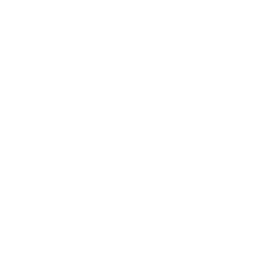
\includegraphics[scale=1]{assets/branding/opa0}
    \vspace{-5.75cm}\\
    {\adjustbox{scale=2.5}{\color{TealDarkCyan}\;I.\;Introduction}}
    \vspace{.25cm}
    \begin{minipage}{.78\textwidth}
      \scriptsize\color{Ink}
      \textbf{Big picture.}\;
      The syndrome of a linear code is a simple linear map — and it is both the key to perfect decoding and the source of a hard cryptographic problem.\\[.2cm]
      \textbf{Details to watch.}\;
      parity-check matrix, syndrome, algebraic structure, NP-hardness, quasi-cyclic.
    \end{minipage}
    {\ }\vspace{2.1cm}\\
    \bigskip
  \end{center}
\end{frame}

%--- Two faces of one object ---
\begin{frame}{\textbf{I. Introduction}}{The Same Object, Two Different Questions}
\small
\begin{columns}[T,onlytextwidth]
\begin{column}{.48\textwidth}
\textcolor{TealDarkCyan}{\textbf{Face 1: Reliable Communication}}
\begin{itemize}
  \item A linear code $\code\le\F_q^n$ adds \emph{known} redundancy.
  \item Channel adds an \emph{unknown} error $\vect e$.
  \item Syndrome $\vect s = \mat H\vect e^T$ reveals $\vect e$.
  \item \textbf{Goal}: recover $\vect e$ quickly — and then correct it.
\end{itemize}
\end{column}
\begin{column}{.48\textwidth}
\textcolor{TealDarkCyan}{\textbf{Face 2: Public-Key Cryptography}}
\begin{itemize}
  \item A random $\mat H$ hides a \emph{secret} sparse $\vect e$.
  \item Adversary sees only $\mat H$ and $\vect s = \mat H\vect e^T$.
  \item No algebraic shortcut exists for a random $\mat H$.
  \item \textbf{Goal}: make recovery computationally infeasible.
\end{itemize}
\end{column}
\end{columns}
\bigskip
\begin{center}
\begin{tikzpicture}[node distance=.72cm]
  \node[process,minimum width=2.8cm] (H) {$\mat H\in\F_q^{r\times n}$\\[-1pt]\scriptsize parity-check matrix};
  \node[process blue,  right=1.4cm of H]  (synd)  {syndrome\\$\vect s=\mat H\vect e^T$};
  \node[process amber, above right=.4cm and 1.4cm of synd] (easy)
    {structured $\mat H$\\$\Rightarrow$ fast decoder};
  \node[process red,   below right=.4cm and 1.4cm of synd] (hard)
    {random $\mat H$\\$\Rightarrow$ NP-hard};
  \draw[flow]       (H)     -- (synd);
  \draw[flow amber] (synd.north east) -- (easy);
  \draw[flow red]   (synd.south east) -- (hard);
\end{tikzpicture}
\end{center}
\end{frame}

%--- The decoding gap ---
\begin{frame}{\textbf{I. Introduction}}{The Decoding Gap}
\scriptsize
\begin{columns}[T,onlytextwidth]
\begin{column}{.56\textwidth}
\defbox[Q. Why does structure matter so much?]{
\textbf{Hamming code.}\;
For $\mat H_3\in\F_2^{3\times 7}$ — columns are all nonzero binary vectors of length 3 —
the syndrome $\vect s = \mat H_3\vect e^T$ \emph{is} the binary address of the error position.
Decoding is a single look-up: $O(1)$ time.

\medskip
\textbf{Random code.}\;
For a random $\mat H\in\F_2^{r\times n}$, the same equation $\mat H\vect e^T = \vect s$ with $\wt(\vect e)=w$
defines the \textbf{Syndrome Decoding Problem}.
The best algorithms run in time $\approx 2^{0.054n}$ — exponential for large $n$.

\medskip
\textbf{What changes?}\;
Nothing in the equation.
Everything in the matrix structure.}
\end{column}
\begin{column}{.40\textwidth}
\begin{center}
\begin{tikzpicture}[scale=.64]
  % Axis: structure on x, decoding cost on y
  \draw[->,Ink!60] (-.2,0) -- (4.5,0)
    node[right,tiny label]{structure};
  \draw[->,Ink!60] (0,-.2) -- (0,3.6)
    node[above,tiny label]{decoding cost};
  % Curve: high cost at left (random), near zero at right (structured)
  \draw[TealDarkCyan,thick,domain=0.2:4.0,samples=40]
    plot (\x, {3.2*exp(-0.9*\x)});
  % Annotations
  \fill[ErrorRed] (0.35,2.55) circle (2.8pt);
  \node[right,tiny label,ErrorRed!80] at (0.5,2.7) {random: $2^{0.054n}$};
  \fill[GoodGreen] (3.5,0.15) circle (2.8pt);
  \node[right,tiny label,GoodGreen] at (3.6,0.3) {Hamming: $O(1)$};
  \fill[BlueCode] (2.1,0.65) circle (2.8pt);
  \node[right,tiny label,BlueCode] at (2.2,0.85) {QC: $2^{0.054m}$};
  \node[caption text,align=center] at (2.2,-0.65)
    {more algebraic structure $\to$ faster decode};
\end{tikzpicture}
\end{center}
\end{column}
\end{columns}
\end{frame}

%--- The central characters ---
\begin{frame}{\textbf{I. Introduction}}{The Central Characters}
\small
\begin{center}
\renewcommand{\arraystretch}{1.28}
\begin{tabular}{>{\bfseries}p{.22\textwidth}p{.35\textwidth}p{.30\textwidth}}
\toprule
Code family & Structure & Decoding \\
\midrule
Hamming $[2^r-1,2^r-1-r,3]_2$ & Projective parity checks & Syndrome = error address; $O(1)$ \\
Cyclic (BCH, RS) & Polynomial ideal in $R_n$ & Root syndromes; polynomial-time \\
QC-MDPC (BIKE) & Circulant blocks in $R_m^\ell$ & Iterative bit-flipping; probabilistic \\
Random linear code & None & SDP; best known $2^{0.054n}$ \\
\bottomrule
\end{tabular}
\end{center}
\bigskip
\textbf{The pattern.}
More algebraic structure enables a more direct decoder —
and makes the code unsuitable as a cryptographic primitive.
Random codes have no efficient decoder and are the right hardness engine.
\end{frame}

%--- Roadmap ---
\begin{frame}{\textbf{I. Introduction}}{Roadmap: A Four-Act Story}
\small
\begin{center}
\begin{tikzpicture}[node distance=.6cm]
  \node[process,minimum width=3.2cm,align=center]
    (act1) {\textbf{Act I (here)}\\Introduction\\Two faces of a syndrome};
  \node[process blue,right=.85cm of act1,minimum width=3.2cm,align=center]
    (act2) {\textbf{Act II}\\When Decoding\\Is \emph{Easy}\\(Hamming, Cyclic)};
  \node[process amber,right=.85cm of act2,minimum width=3.2cm,align=center]
    (act3) {\textbf{Act III}\\When Decoding\\Is \emph{Hard}\\(SDP, NP-complete)};
  \node[process red,right=.85cm of act3,minimum width=3.2cm,align=center]
    (act4) {\textbf{Act IV}\\The Compromise\\(QCSD, BIKE, HQC)};
  \draw[flow]       (act1) -- (act2);
  \draw[flow blue]  (act2) -- (act3);
  \draw[flow amber] (act3) -- (act4);
\end{tikzpicture}
\end{center}
\bigskip
\begin{columns}[T,onlytextwidth]
\begin{column}{.48\textwidth}
\textcolor{TealDarkCyan}{\textbf{What we build up}}
\begin{itemize}
  \item Linear codes, syndromes, cosets
  \item Hamming: perfect single-error correction
  \item Cyclic: polynomial-ring structure
\end{itemize}
\end{column}
\begin{column}{.48\textwidth}
\textcolor{TealDarkCyan}{\textbf{Where we arrive}}
\begin{itemize}
  \item SDP: NP-complete for random $\mat H$
  \item QCSD: structured but still hard
  \item BIKE and HQC: compact PQC systems
\end{itemize}
\end{column}
\end{columns}
\end{frame}
